\subsection{The same fall in directional share can conceal opposite changes in lead--lag structure}

The MI result suggests a more general question about paired statistics. Can a change in agreement be decomposed into the contributions of its two profiles? For temporal orientation there is an exact example. At a fixed delay, compare a matrix of lagged correlations with its transpose. A pair can share a large lagged correlation in both directions. Only the difference between those directions distinguishes which signal leads. The fraction of edge variation in that difference is exactly $(1-z)/2$. Time-reversal contrasts have previously distinguished brain states in these same macaques \cite{deco2022}. Here we separate the magnitude of the asymmetric component that recurs across windows from its share of all repeatable lagged structure.

At 20 ms, the mean repeatable asymmetric share fell under each drug, by 4.2--5.4 percentage points, and by 6.3 points in sleep (\cref{fig:lag}). Yet its absolute contribution rose under ketamine on all four dates and fell under propofol on all four dates and under the combination on all eleven. The ketamine and propofol dates included the same two animals. Under ketamine the symmetric component grew enough to dilute a growing asymmetric component. Under propofol the asymmetric component itself diminished. All-channel estimates and disjoint bipolar derivations preserved these three directions by date. When Fourier amplitudes were fixed to each date's wake spectrum, the absolute change remained positive on three of four ketamine dates and negative on every propofol and combination date. The group mean share then rose under ketamine. Thus the uniform fall in share depended on spectral weighting, whereas the drug contrast in repeatable asymmetric structure partly survived its removal.

This finding is exploratory and time-scale specific. At 40 ms the combination's mean absolute change became slightly positive on the primary montage. Eyes-open wake also changed the share, and recovery was incomplete for several agents. The ketamine increase was substantially larger in Chibi than in George. These properties make the measure a descriptor of temporal organisation at a stated lag. Inferring a propagation pathway would require additional spatial or interventional evidence.

We also applied the same 20-ms readout to awake and sustained isoflurane EEG in the independent mouse dataset, using the first eligible date per animal and all retained channels. With common-average reference the mean share fell from $5.48\%$ to $1.45\%$ (16/17 mice down), and mean repeatable asymmetric energy fell from $0.00341$ to $0.00097$ (16/17 down). With the as-recorded reference, the share fell in 17/17, but absolute energy fell in only 11/17. Thus the relative reorganisation extends to this burst-suppressed state. The absolute component is more reference-sensitive, and this comparison cannot establish an effect independent of bursting.

\begin{figure}[htbp]
\centering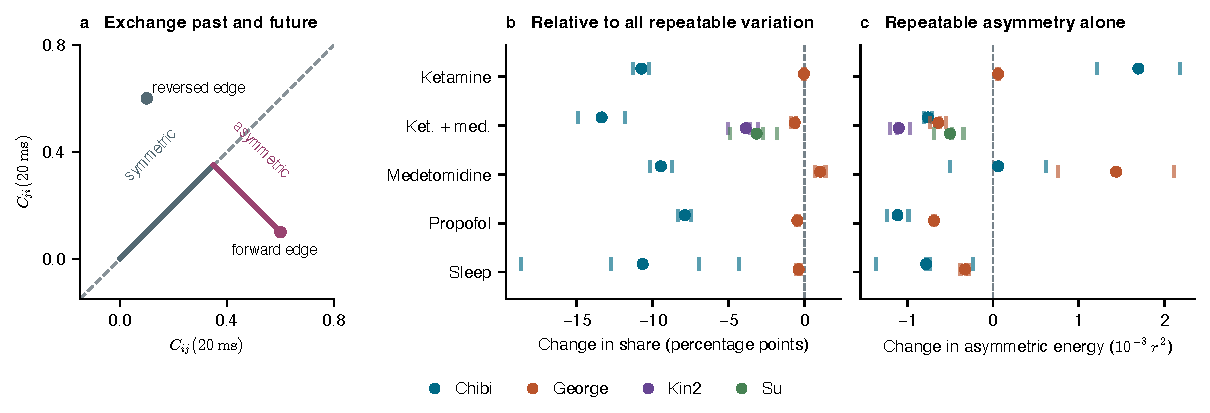
\includegraphics[width=\linewidth]{lag-reciprocity}
\caption{\textbf{A lag profile has two distinguishable components.} (a) For one illustrative pair, equal forward and reverse correlations lie on the diagonal. Its displacement perpendicular to that diagonal measures orientation asymmetry. (b) State minus eyes-closed wake for the share of lagged variation carried by recurring asymmetric edges. (c) The same contrast for absolute repeatable asymmetric energy. Short ticks are dates; dots are animal means. The same two animals contribute ketamine and propofol dates. Panels b and c use a 20-ms lag and common-average reference.}
\label{fig:lag}
\end{figure}
